\section{Arquitetura da Solução} \label{sec:arquitetura_solucao}

O sistema está representado na Figura \ref{fig:arquitetura}, encontra-se dividido em três camadas: Simulador, \textit{Back-end} e \textit{Front-end}. O fluxo de informação ocorre de forma descendente no que toca à telemetria, e de forma bidirecional na interação com o cliente.

\begin{figure}[htb]
	\centering
	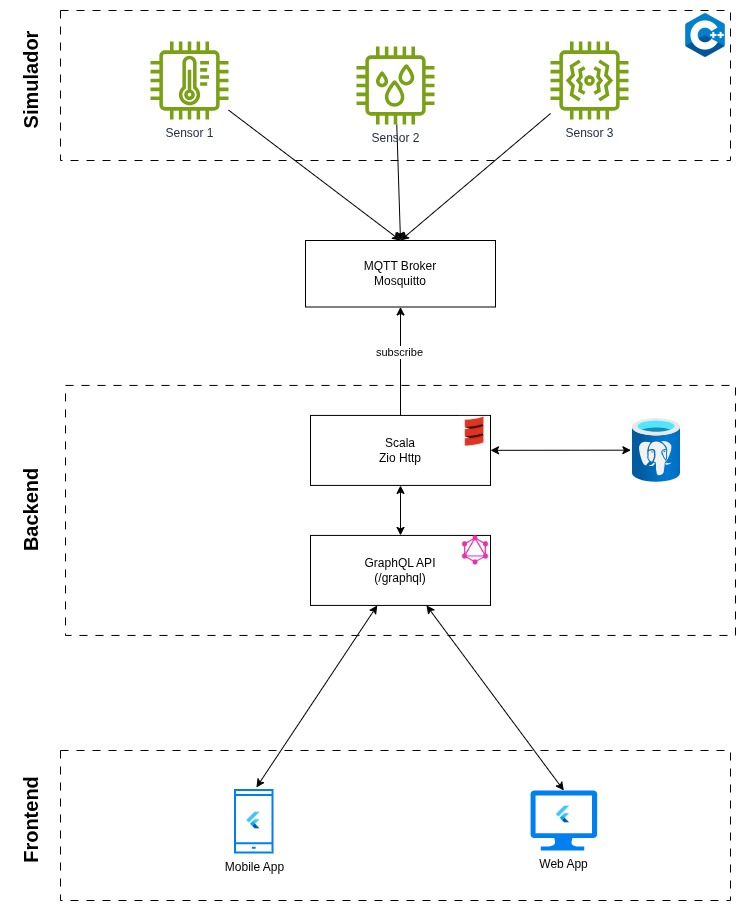
\includegraphics[width=0.6\textwidth]{imagens/architeture.jpg}
	\caption{Diagrama de Arquitetura de Alto Nível}
	\label{fig:arquitetura}
\end{figure}


\subsection{Camada de Simulação (Ingestão de Dados)}
Na camada superior encontram-se os componentes desenvolvidos em C++, responsáveis por mimetizar o comportamento de dispositivos físicos num ambiente IoT (Sensores 1, 2 e 3). Estes simuladores geram medições contínuas (como temperatura e humidade) e atuam como produtores (\textit{publishers}). Os dados gerados são enviados para um \textit{Broker} MQTT (neste caso, o \textit{Mosquitto}) seguindo a especificação Sparkplug B. Esta convenção tira partido de \textit{Protocol Buffers} (Protobuf) para a serialização binária dos dados, um padrão que reduz drasticamente o tamanho do \textit{payload} e acelera a comunicação. A escolha do MQTT e do Sparkplug B justifica-se por constituir o ecossistema padrão e mais eficiente na comunicação \textit{machine-to-machine} (M2M) na indústria.

\subsection{\textit{Back-end} (Processamento e Persistência)}
O Back-end, desenvolvido em Scala com recurso à biblioteca \textit{ZIO} e \textit{ZIO HTTP}. O fluxo de operações decorre da seguinte forma:
\begin{itemize}
	\item \textbf{Subscrição e Processamento:} O servidor Scala atua como cliente do \textit{broker} MQTT, subscrevendo os tópicos dos sensores. À medida que as mensagens chegam, entram numa \textit{pipeline}, onde a informação é validada e filtrada. % TODO ainda não sei se tenho validação (deve entrar tudo)
	\item \textbf{Armazenamento de Histórico:} O \textit{back-end} comunica com uma base de dados relacional PostgreSQL para persistir os dados processados.
	\item \textbf{Interface de Comunicação:} Para servir as aplicações cliente, o servidor expõe uma API GraphQL.
\end{itemize}

\subsection{\textit{Front-end} (Visualização Web e Mobile)}
Na camada de \textit{Front-end} encontram-se a aplicação para dispositivos móveis e a aplicação \textit{Web}, ambas desenvolvidas na \textit{framework} Flutter a partir de um \textit{package} partilhado entre as duas, evitando duplicação desnecessária de código. 

Estas aplicações comunicam exclusivamente com o serviço de \textit{Back-end} através da API GraphQL. Esta ligação reflete-se na arquitetura através das setas bidirecionais, pois o cliente não realiza apenas \textit{Queries} (pedidos HTTP) para obter o histórico guardado no PostgreSQL. Crucialmente, as aplicações cliente estabelecem ligações persistentes via \textit{WebSockets} (através de \textit{Subscriptions} GraphQL) com o servidor Scala. Isto garante que sempre que um novo evento passa pela \textit{pipeline} do \textit{back-end}, os \textit{dashboards} Flutter são atualizados em tempo real, sem necessidade de \textit{polling} constante.

% TODO validar mais tarde se isto está correto
\subsection{Fluxo de Dados e Interação}
Todo o fluxo de dados da aplicação está descrito na Figura \ref{fig:sequencia}, que demonstra o comportamento dinâmico e a interação em tempo real entre as três camadas descritas anteriormente.

\begin{figure}[htb]
	\centering
	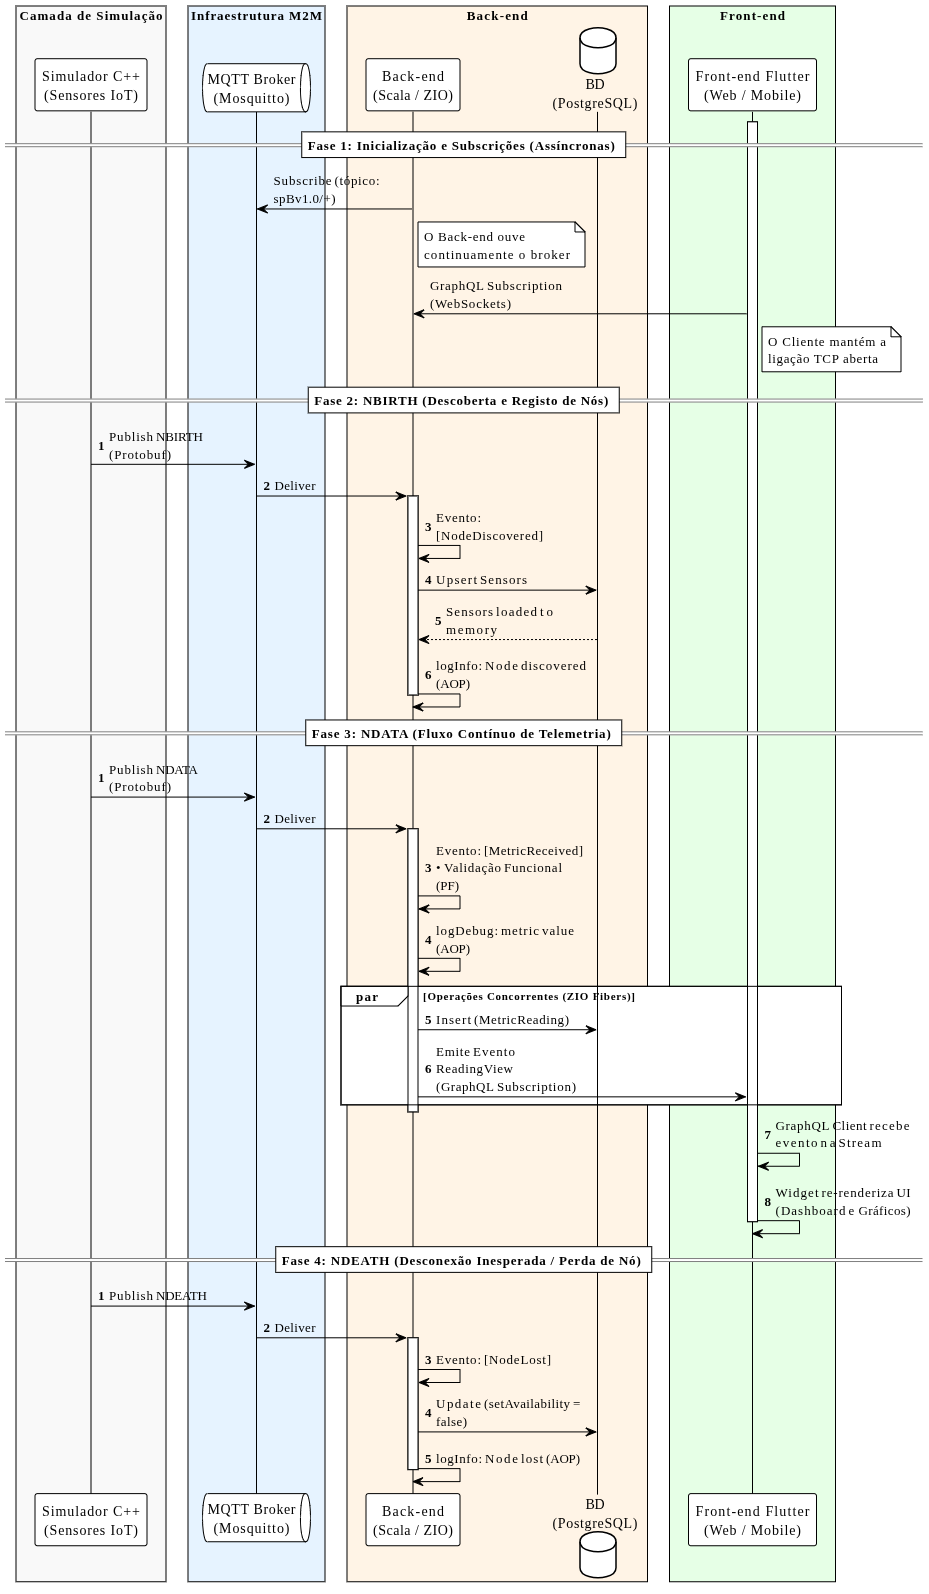
\includegraphics[width=0.8\textwidth]{imagens/messages_sequence_diagram.png}
	\caption{Diagrama de Sequência ilustrando o fluxo de eventos em tempo real.}
	\label{fig:sequencia}
\end{figure}

O processo inicia-se de forma assíncrona, com o servidor Scala e a aplicação Flutter a estabelecerem as respetivas subscrições. A partir desse momento, o sistema entra num ciclo contínuo onde a telemetria publicada pelo simulador é consumida pelo \textit{Back-end}. Tirando partido da concorrência nativa da biblioteca ZIO (\textit{Fibers}), o servidor persiste o registo na base de dados em simultâneo com a emissão do evento para o \textit{Front-end}, garantindo que a interface do utilizador é atualizada instantaneamente.